% The section about the project architecture, preparing the implementation
% @author Kalvin Döge
%


\section{Projektarchitektur}\label{sec:projectarchitecture}

Die Architektur dieses Modells ist wie folgt:

\begin{figure}[h]
    \centering
    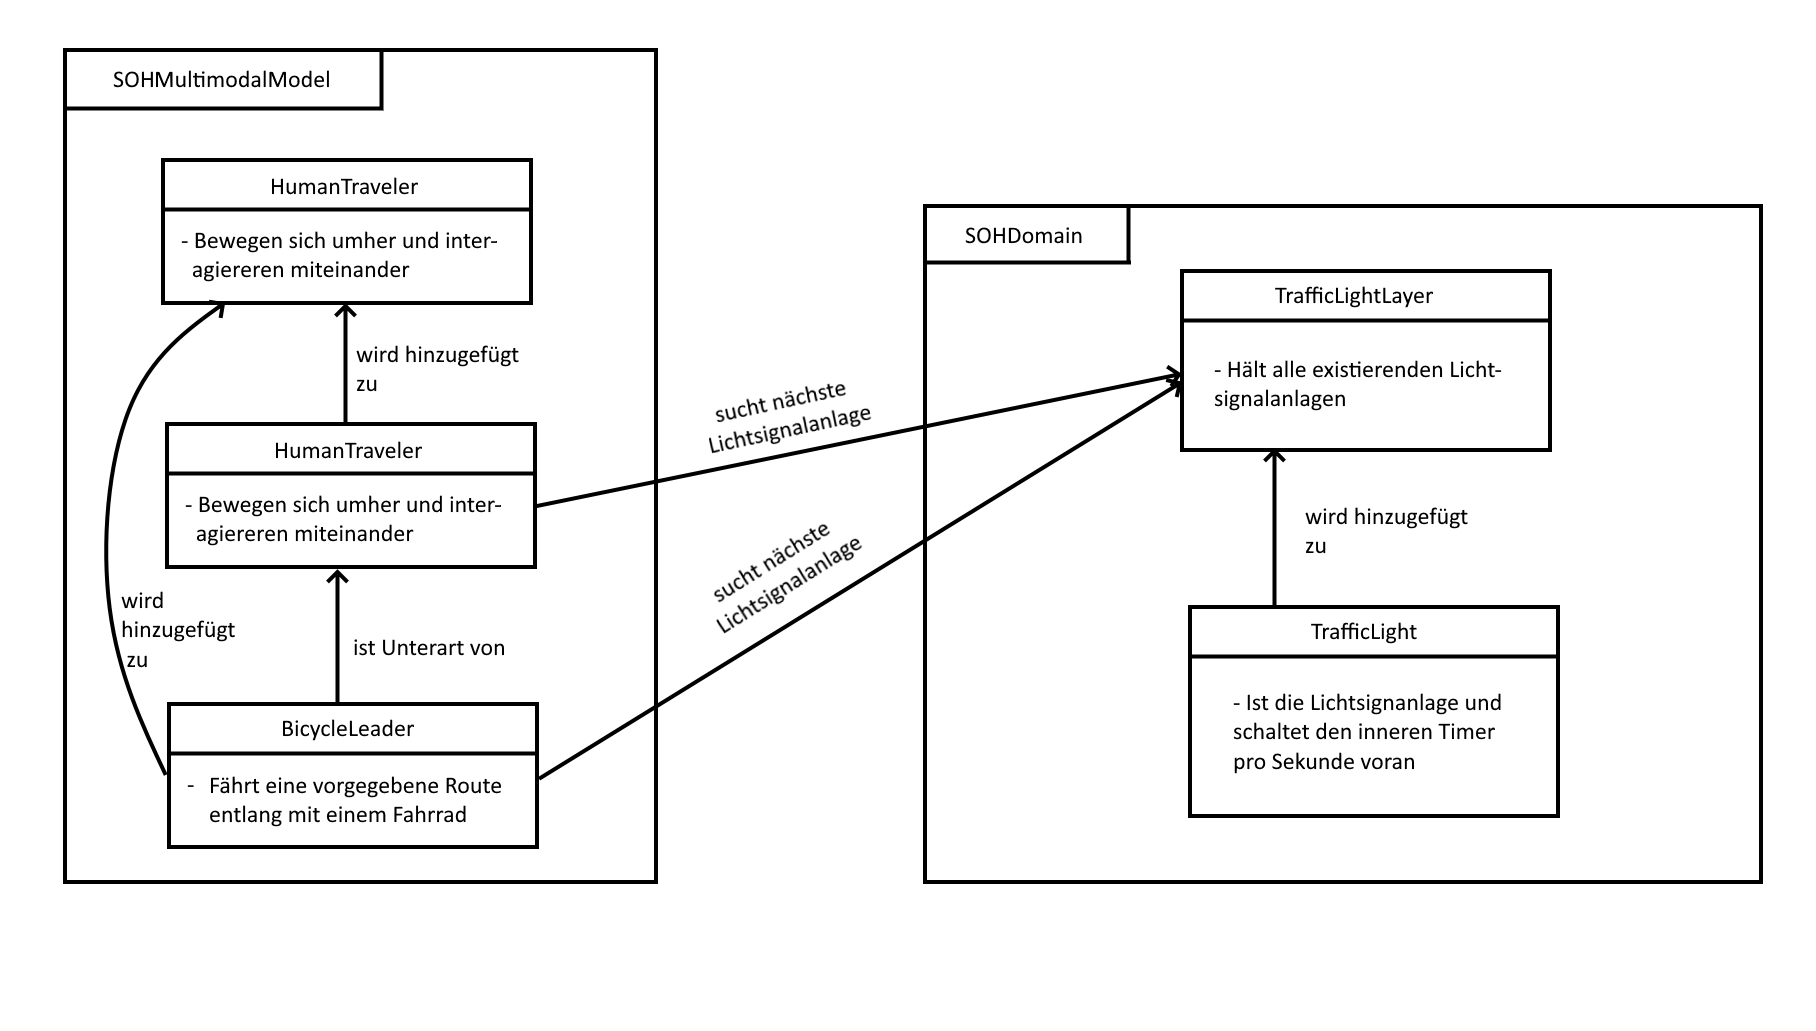
\includegraphics[width=0.75\textwidth]{architecture}
    \caption{Klassendiagramm der Agenten und Entitäten}
    \label{fig:class-diagramm}
\end{figure}

\code{HumanTraveler} werden jede Stunde erschaffen und zu ihrem \code{HumanTravelerLayer} hinzugefügt.
Die erschaffenen \code{HumanTraveler} bewegen sich auf dem \code{HumanTravelerLayer}, auf der sie mit anderen Agenten interagieren können.

Zu jeder vollen Stunde wird ein \code{BicycleLeader} in dem \code{HumanTravelerLayer} hinzugefügt und erhält dann über die \code{BicycleLeaderRoute} die zugewiesenen Routenpunkte, die dieser abfahren muss.

Die \code{TrafficLight}s werden zu Beginn vollständig in die Simulation geladen und zu einem \code{TrafficLightLayer} hinzugefügt.
Danach stehen sie jedem \code{HumanTraveler} zur Verfügung als Referenz, sobald diese wiederum erstellt werden.
\code{BicycleLeader} sind dabei eine Unterklasse der \code{HumanTraveler} und haben somit auch Zugriff auf den \code{TrafficLightLayer}.


Ein \code{TrafficLight} besitzt die folgenden Eigenschaften: Die Position angegeben als \code{Longitude} und \code{Latitude}, eine zufällig zugewiesene GUID namens ,,\code{EntityID}``, die Länge der Rot- und Grünphase als \code{LengthPhaseRed} und \code{LengthPhaseGreen}, die aktuell verstrichene, interne Zeit als \code{CurrTime}, die aktuelle Lichtsignalphase \code{CurrPhase} und zuletzt noch die wartenden Agenten über eine Warteschlange: \code{WaitingRoadUsers}.

\code{HumanTraveler}s können ein \code{Bicycle}, \code{Car} oder nichts bei sich erschaffen.
Eines dieser Modalitäten ist dann ihr Transportmittel, das \code{Vehicle}.

\code{BicycleLeader} sind identisch zu den \code{HumanTraveler}s, bis auf die Einschränkung, dass sie nur \code{Bicycle} nutzen beziehungsweise zu Fuß zum \code{Bicycle} gehen können.


\code{HumanTraveler} nutzen für das Erreichen ihres Zieles den \code{RouteFinder}, mit der sie eine Route zum Abfahren berechnet bekommen.


\code{TrafficLight}s haben folgende Funktionen, die eine Relevanz für sie selbst oder für andere Agenten in der Simulation haben:

\code{public void Tick()} setzt die innere Zeitschaltung der Ampel fort und damit auch die nächste \code{CarLightSignalPhase}, zum Beispiel von Gelb zu Rot.

\code{public void CheckQueue()} überprüft die aktuelle Warteschlange und entfernt, sobald der Agent nicht mehr warten sollte, ihn aus der Warteschlange.

\code{public Boolean Enter(IAgent IAgent)} fügt den angegebenen Agenten zur Warteschlange hinzu, sollte die aktuelle \code{CarLightSignalPhase} Rot sein.

\code{public Boolean CanPass(IAgent IAgent)} gibt einen Wahrheitswert zurück, ob der Agent sich überhaupt in der Nähe der Ampel befindet und wenn ja, ob dieser einfach vorbeifahren kann wegen eines grünen Lichtsignales und keinen wartenden, anderen Agenten.

\code{public Boolean IsQueued(IAgent IAgent)} überprüft und gibt einen Wahrheitswert zurück, ob der Agent noch in der Warteschlange notiert ist.

